\clearpage
\subsubsection{Pre-Test Loop} % (fold)
\label{sub:pre_test_loop}

The Pre-Test Loop is a looping statement that allows code to be run 0 or times. The loop checks the condition at the start, and if the condition is True the loop's body is executed. At the end of the loops body the computer jumps back to the condition, checking it again to determine if the loop's body should execute again. If the condition is False when it is checked the loop jumps ends, and control jumps to the next statement in the code.

\begin{figure}[h]
   \centering
   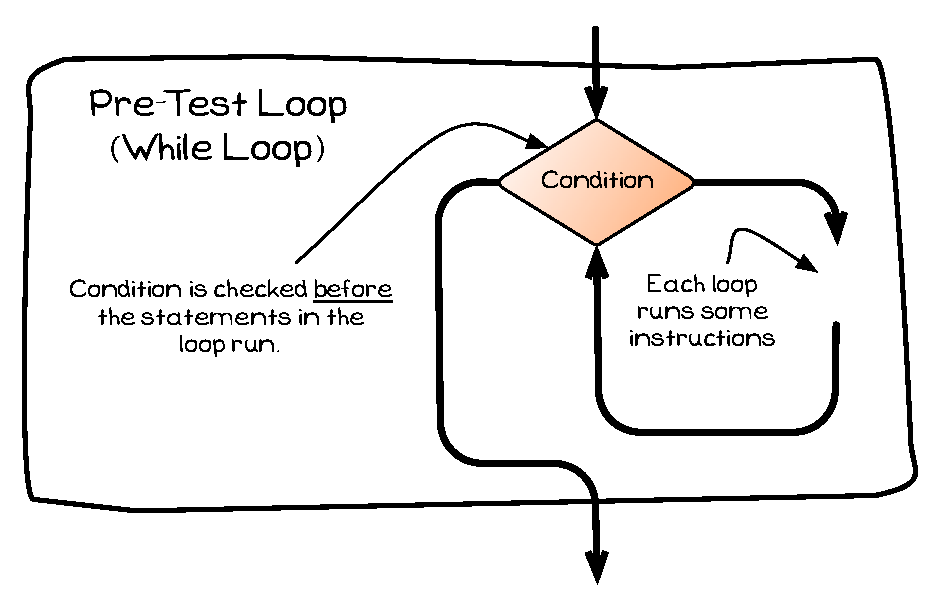
\includegraphics[width=\textwidth]{./topics/control-flow/diagrams/PreTestLoop} 
   \caption{The Pre-Test Loop checks the condition, then runs the loop's body}
   \label{fig:looping-pre-test}
\end{figure}

\mynote{
\begin{itemize}
  \item A pre-test loop is an \textbf{action}, creating a loop in the code's sequence of instructions.
  \item The standard pre-test loop is the \textbf{while statement}.
  \item A pre-test loop allows instructions to be run 0 or more times.
  \item The condition is checked when the loop's code is entered, and it is checked again at the end of each loop.
\end{itemize}
}


% subsection post_test_loop (end)